\documentclass[12pt]{article}
\usepackage{amsmath}
\usepackage{csvsimple}
\usepackage{graphicx}
\graphicspath{ {./../images/} }
\usepackage{hyperref}
\usepackage[latin1]{inputenc}
\usepackage{listings}

\DeclareMathOperator{\Tr}{Tr}

\lstset{
  columns=fullflexible,
  breaklines=true,
  }

\twocolumn

\title{Local Assortativity in Networks with Unbalanced Classes}
\author{Rebecca Cohen}

\begin{document}
\maketitle
\section{Introduction}

In many network datasets, edges may be more, or less, frequent between pairs of nodes that share a common attribute.  To measure this tendancy on a network with a discrete attributes, we use the normalized modularity score
 \begin{equation}
   r = \frac{Q}{Q_{max}} = \frac{\sum_g e_{gg} - \sum_g a_g^2} {1 - \sum_g a_g^2}
 \end{equation} \cite{newman:2003}
 
 where $e_{gg}$ is the fraction of edges that connect nodes of class $g$, and $a_g$ is the fraction of edges attached on either side to nodes of class $g$.  This statistic provides a global summary of the relation between edges and attribute values across the network.  
 
However, this metric will not capture the variation that occurs within the network.  To capture a more nuanced representation of the assortative behavior in the neighborhood of a fixed node $i$, Peel et al. have proposed a local assortativity measure

\begin{equation}
  r_\ell = \frac{1}{Q_{max}} \sum_g (e_{gg}(\ell) - a_g^2)
\end{equation}

where $e_{gg}(\ell)$ is the fraction of edges connecting nodes in class $g$, weighted by the importance of each endpoint in the neighborhood of $\ell$.  

Personalized PageRank is a popular measure of local node importance in which $w_\alpha(i; \ell)$ is the stationary probability that a random walker beginning at $\ell$ will be at $i$, assuming they teleport back to $\ell$ with probability $1-\alpha$.  Some sources reverse the roles of $\alpha$ and $1 - \alpha$ \cite{chen:2020}, but this paper will follow the convention used by Peel et al \cite{Peel:2018}.  When $\alpha$ is close to 0, the bulk of weight is in the immediate neighborhood of $\ell$, while values closer to 1 produce something closer to the global assortativity.  More formally, the personalized PageRank vector $\vec{w}_\alpha$ is the unique solution to
\begin{equation}
  \vec{w}_\alpha^T = (1 - \alpha) \vec{\pi}^T + \alpha \vec{w}_\alpha^T \mathbf{P}
\end{equation}

where $\vec{\pi}$ is the unit vector in the direction of $\ell$ and $\mathbf{P}$ is the transition matrix; $\mathbf{P}_{ij}$ denotes the probability that a random walker currently at node $i$ will arrive at node $j$ after randomly following one edge.

To summarize the behavior across multiple scales, we use the TotalRank

\begin{equation}
  w_{multi}(i; \ell) = \int_0^1 w_\alpha(i; \ell) d\alpha
\end{equation} \cite{boldi:2005} \cite{Peel:2018}

and define
\begin{equation}
  e_{gg}(\ell) = \sum_{i: z_i \in g} \sum_{j: z_j \in g} w_{multi}(i; \ell) \frac{\mathbf{A}_{ij}}{k_i}
\end{equation} \cite{Peel:2018}

where $\mathbf{A}$ is the adjacency matrix of the network, $\vec{k}$ is the degree vector, and $\vec{z}$ is the attribute vector.

Peel et. al find considerable variation in $r_\ell$ on both random and empirical networks.  However, it is not obvious whether local differences in assortativity are the result of differences in the probability of nodes forming in-group vs. out-group edges, or whether there may be other factors that influence the distribution of $r(\ell)$.

This paper will analyze the distribution of $r(\ell)$ with respect to class size.  We find that otherwise comparable nodes in larger classes tend to have higher $r(\ell)$ scores on both assortative and disassortative networks.  We develop a theoretical prediction of $r(\ell)$ based on a DC-SBM null model and use numerical experiments to validate its predictions.

\section{Methods}
We can test the influence of class size on local assortativity, using random graphs in which there is no fine-grained assortative structure.  We consider two different null models, the Erdos-Renyi random graph, which has no assortatitive structure, and a simple stochastic block model (SBM) with equal in- and out-group pairing probabilities for all classes of nodes.

The Erdos-Renyi random graphs in this experiment had $N=800$, $p=0.075$, while the SBM had 2 blocks of varying sizes, with $N=800$, with an in-group pairing probability of 0.1 and out-group pairing probability of 0.05.  On both models, nodes were assigned to one of two classes, with the size of the smaller class varying between 10 and 400 by units of 10.  For each choice class size, 20 trials were run on different random graphs and the mean $r_\ell$ was recorded for each class, as was the global assortativity.

We then derive an estimate of the expectation of $r_\ell$ on a network with global assortative structure but no fine-grained variation within each class.  To test the estimates, we fix the proportional sizes of 10 classes as well as in-group and out-group pairing probabilities.  For varying sizes of network, we generate 50 DC-SBM random networks and compare the mean $r_\ell$ values within each class with the estimate.  We also examine the distribution of $r_\ell$ within each class.  

\section{Results}
\subsection{Class Size and Local Assortativity}

Figure 1 shows the results of the initial experiment.  On both null models, the larger class consistently had higher $r(\ell)$ scores than the smaller one.  The steep dropoff in $r(\ell)$ as the smaller class size decreases is striking in both experiments.  Neither network had disassortative structure, yet as the size of the smaller group approaches 0, $r(\ell)$ approaches $-\infty$.  The precipitous drop in score has to do with the normalization term.  Without loss of generality, suppose the largest group is group 1.  As the size of group 1 approaches the entire dataset, $a_1 \to 1$, so
\begin{equation}
  Q_\text{max} = 1 - \sum_g a_g^2 \to 1 - 1 = 0 
\end{equation}

\begin{figure}[ht!]
  \includegraphics[width=0.5\textwidth]{erdos_renyi_{date_str}.png}
  \includegraphics[width=0.5\textwidth]{unbalanced_sbm_2021_11_30_13_01.png}
  \caption{Distribution of $r(\ell)$ on Erdos-Renyi random graphs (top) and SBM's (bottom).  Error bars indicate the standard deviation of the mean $r(\ell)$ for each class between trials.}
\end{figure}

The normalization term explains the magnitude of the decline in $r_\ell$, but to understand why it is negative to begin with we must consider what happens to $e_{gg}(\ell)$ as class sizes become increasingly unbalanced.  Consider a node $\ell$ in group 1, the larger group.  TotalRank will assign a higher weight to node $\ell$ than to any other node, thus edges connecting node $\ell$ to other nodes in group 1 will be given the most weight in $e_{11}(\ell)$, leading to a higher proportion of in-group edges than expected even when there is no assortative structure.  Internal edges in group 2 will be given weight less than $a_2^2$ but these are a smaller fraction of the network so this different will be outweighted by the results from group 1.

Conversely, if we take $\ell$ in group 2, the smaller group, then $e_{22}(\ell)$ will be greater than $a_2^2$, but this will be outweighed by the large defecit in $e_{11}$ as none of the top-weighted edges can be internal to group 1.

We can see from the SBM experiment that global, as well as local, assortativity scores depend on class size, reaching a maximum when classes have equal sizes.  While it is tempting to search for class-size correction that could be applied $r(\ell)$, the assumption that a variation on modularity could be independent of class size may be misguided.

\subsection{Baseline Local Assortativity}

In order to draw conclusions about local differences in node pairing behaviors, we would like to be able to distinguish between variance in $r(\ell)$ due to class size vs. fine-grained differences in behavior.  

With two key assumptions, we can calculate $\hat{r}_\ell$, an estimator of $r(\ell)$ for each node under a degree-corrected stochastic block \\model (DC-SBM).

\begin{enumerate}
  \item The degree of every node is equal to its expected degree
  \item The network is fully connected
\end{enumerate}

Assumption 1 allows us to treat node degrees and edge counts as constants.  Without this assumption, both $e_{gg}(\ell)$ and $a_g$ are the ratios of two Poisson random variables, and it is theoretically possible for the denominator to equal 0, rendering these expectations undefined.  More work is needed to develop probabilistic bounds on the error, but numerical simulations support the utility of this naive appoximation (see figure BLAH).

An alternate framing of this work that may make assumption 1 more palatable is to consider using $\hat{r}_\ell$ as a baseline with which to compare an observed value.  Since the DC-SBM functions as a null model that accounts for the role of degree and blockwise assortativity, we may conceive of $\hat{r}_\ell$ as the expectation of $r_\ell$ on a hypothetical null model that is guaranteed to satisfy both assumptions.  We can calculate the estimate on this hypothetical model even if we do not understand how one could generate it.

Assumption 2 will become necessary when we compute transition probabilities for the blockwise personalized PageRank. 

Before deriving $\hat{r}_\ell$, we must define several variables.  To specify the DC-SBM, we define $N$ equal to the number of nodes in the network and $c$ equal to the number of discrete attributes in the network.  Then $\mathcal{M}$ is a $c \times c$ matrix, with $\mathcal{M}_{gh}$ equal to the target number of edges between class $g$ and $h$.  Block membership is defined with $\vec{z}$, an $N$-dimensional vector such that $z_i$ defines the block to which the $N$th node belongs.  We specify the degree of each node with the degree vector $\vec{k}$, although at times it will be more convenient to work with the block-normalized degree vector $\vec{\gamma}$, which specifies $\gamma_i \in (0, 1]$, the proportion of the edge wealth of block $z_i$ that is attached to node $i$.  \cite{clauset:2021}

In the context of this calculation we treat $\mathbf{A}$ as a random variable that denotes the adjacency matrix of a network generated by our idealized DC-SBM model.  We work with $e_{gg}(\ell)$, $a_g$, $w_\alpha(i; \ell)$, $w_{multi}(i; \ell)$ and $r_\ell$ as defined in equations 1 through 4.

Since every node has its expected degree under assumption 1,
\begin{equation}
  \begin{aligned}
    a_g &= \sum_i \sum_j A_{ij} \delta(z_i, g) \\ 
    &= \sum_i \delta(z_i, g) k_i \\
    &= \sum_h \mathcal{M}_{gh}
  \end{aligned}
\end{equation}

Noteably, $a_g$ is a constant here so 
\begin{equation}
  \hat{r}(\ell) = \frac{\langle e_{gg}(\ell) \rangle - \sum_g \big( \mathcal{M}_{gh} \big)}{1 - \sum_g \big( \mathcal{M}_{gh} \big)}
\end{equation}

To compute the expectation of $e_{gg}(\ell)$, we consider a simplified network in which all nodes within each block are collapsed into a supernode, with edge weights equal to the count of lower-level edges.  Under assumption 1, the mixing matrix $\mathcal{M}$ becomes the adjacency matrix of the collapsed network.  In a typical DC-SBM, these edge weights would be Poisson distributed with mean $\mathcal{M}_{gh}$.

Applying the PPR algorithm to $\mathcal{M}$, we can compute the $c$-dimensional blockwise PPR vector $\vec{w}_\alpha(g; z_\ell)$.  This lower-dimensional vector represents the stationary distribution of the PPR random surfer across each of the $c$ blocks.  This calculation relies on assumption 2, as it requires the nodes within each block to be reachable from anywhere on the network proportional to the transition probabilities of the mixing matrix.

We rely on recent work by Chen et al \cite{chen:2020} relating the nodewise and blockwise and PPR vectors:
\begin{equation}
  \langle w_\alpha (i ; \ell) \rangle = \gamma_i w_\alpha(g; z_\ell)
\end{equation}
Their proof is outside of the scope of this paper, but follows from the lack of any intra-block structure in the DC-SBM.

Using the linearity of both expectation and integration, we find the TotalRank \cite{boldi:2005} \cite{Peel:2018} of node $i$ with respect to $\ell$:
\begin{equation}
  \begin{aligned}
    \langle w_\text{multi} (i ; \ell) \rangle &= \big \langle \int_0^1 w_\alpha(i; \ell) d\alpha \big \rangle \\
    &= \int_0^1 \langle w_\alpha(i; \ell) \rangle d\alpha \\
    &= \gamma_i \int_0^1 w_\alpha(g; z_\ell) d\alpha
  \end{aligned}
\end{equation}

Since $w_\alpha (g;\ell)$ can be computed in just $O(C^2)$, the blockwise PPR can be found cheaply for many choices of $\alpha$ and the integral approximated numerically.  Future work could explore more direct and elegant approaches for computing $w_{multi}$. 

Under assumption 1, $k_i = \theta_i$ for every node, so $k_i$ and $\theta_i$ will cancel in the equation for $\langle e_{gg} (\ell)$, so
\begin{equation}
    \langle e_{gg}(\ell) \rangle = \big \langle \sum_i \sum_j w_\text{multi}(z_i; \ell) A_{ij} \delta(z_i, z_j) \big \rangle\\
\end{equation}

In theory, $w_\text{multi}$ is not independent of $\sum_i \sum_j A_{ij} \delta(z_i, z_j)$, as the existance or nonexistance of each in-group edge has a impact on the blockwise transition matrix.  However, with a sufficiently high mean degree, the results will be close to independent, so we approximate
\begin{equation}
  \begin{aligned}
    \langle e_{gg}(\ell) \rangle &= \big \langle w_\text{multi}(g; \ell) \big \rangle \big \langle \sum_i \sum_j A_{ij} \delta(z_i, z_j) \big \rangle \\
    &= w_\text{multi}(g; \ell) \mathcal{M}_{gg}
  \end{aligned}
\end{equation}

Substituting the expection of $\langle e_{gg}(\ell)\rangle$ back into equation NUMBER, we find

\begin{equation}
  \langle r(\ell) \rangle = \frac{\mathcal{M}_{gg} w_\text{multi}(g; \ell) - \sum_g \big( \mathcal{M}_{gh} \big)}{1 - \sum_g \big( \mathcal{M}_{gh} \big)}
\end{equation}

Equation NUMBER depends only on the mixing matrix and blockwise PPR vector.  This means that $\langle r(\ell) \rangle$ will be the same for every element of each block, regardless of its degree.  It also means that we can compute $\langle r(\ell) \rangle$ directly from the mixing matrix.

\section{Numerical Experiments}
The calculation above relied on some highly unrealistic but conveninent assumptions about the DC-SBM.  To test how well these predictions work in practice, we generate networks using a DC-SBM and compare the distribution $r_\ell$ scores with the theoretical prediction from equation NUMBER.

For these experiments, we select a heterogeneous distribution of block sizes and degree distributions.  We keep the ratios of block sizes roughly fixed between trials, with adjustments to account for rounding.  We generate both assortative and disassortative networks, keeping in-group and out-group probability of an edge existing constant between classes, so the only structural difference between different classes is the size of the class. 

\begin{figure}[h!]
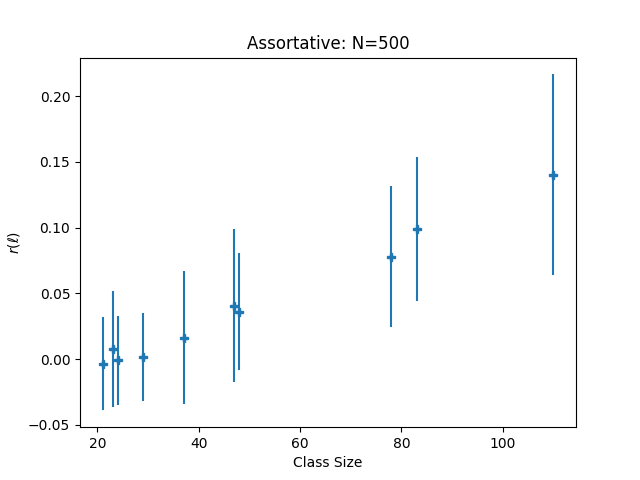
\includegraphics[width=0.5\textwidth]{assortative_N_500.png}
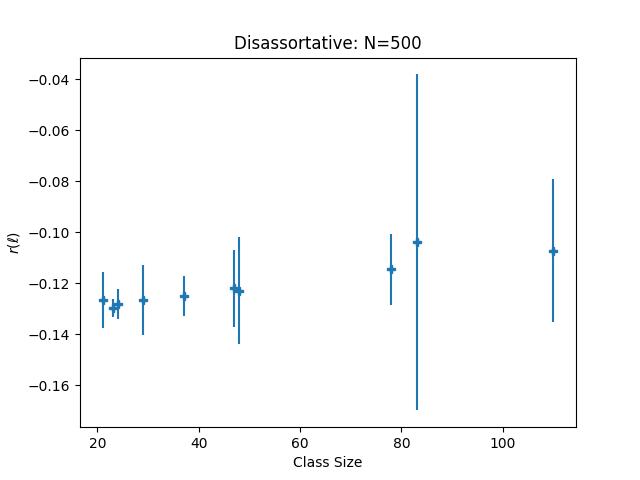
\includegraphics[width=0.5\textwidth]{disassortative_N_500.png}
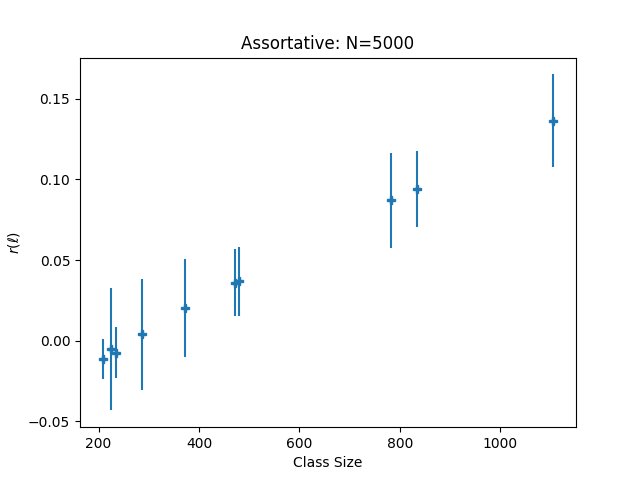
\includegraphics[width=0.5\textwidth]{assortative_N_5000.png}
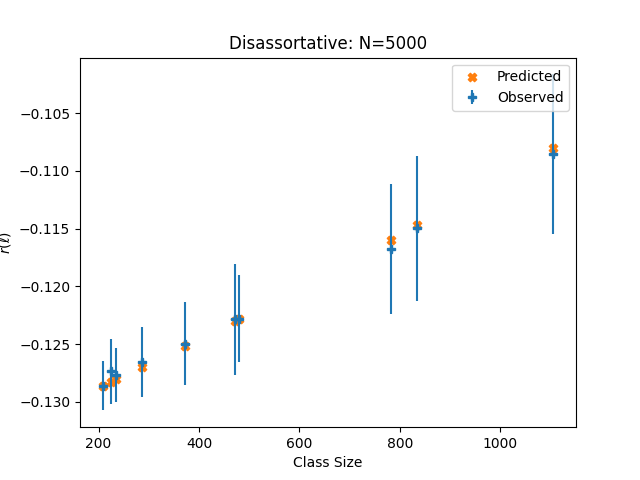
\includegraphics[width=0.5\textwidth]{disassortative_N_5000.png}
\caption{Distribution of $r(\ell)$ on DC-SBM random networks.  Errorbars show the standard deviation within each class}
\end{figure}

Figure NUMBER shows the distribution of $r_\ell$ within each class on a single DC-SBM for both assortatiive and disassortatiive nettworks.  Mean scores appear close to the theoretical prediction and the standard deviation decreases as the size of the network grows.  These networks were constructed in such a way that larger networks had higher mean degree, which decreases the impact of random fluctuations due to a small number of edges.  

\begin{figure}[h!]
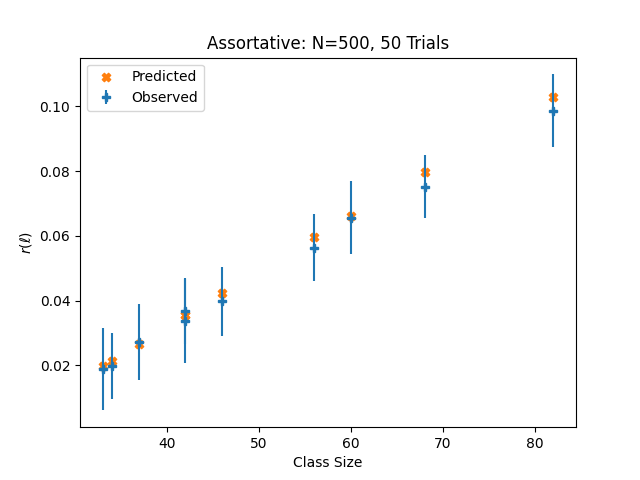
\includegraphics[width=0.5\textwidth]{assortative_N_500_trials_50.png}
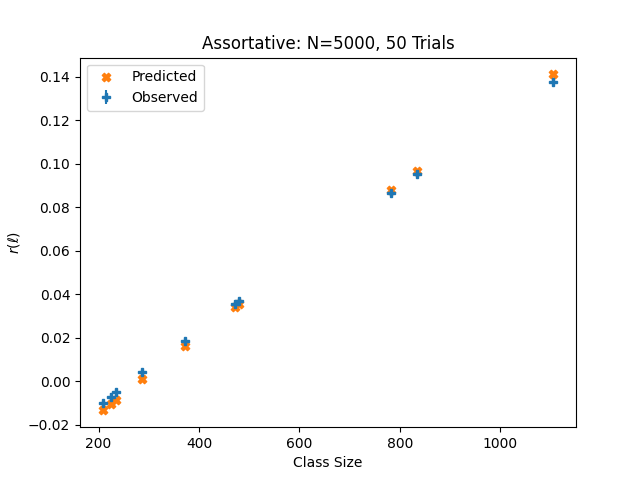
\includegraphics[width=0.5\textwidth]{assortative_N_5000_trials_50.png}
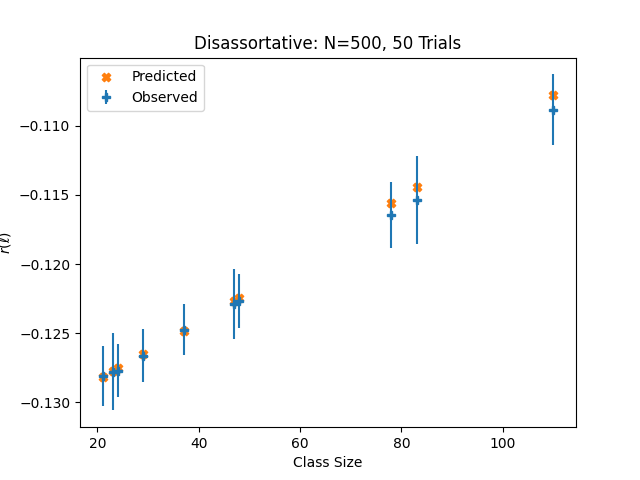
\includegraphics[width=0.5\textwidth]{disassortative_N_500_trials_50.png}
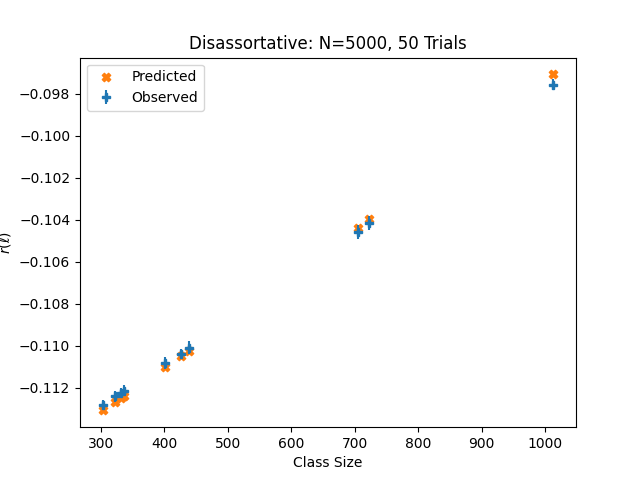
\includegraphics[width=0.5\textwidth]{disassortative_N_5000_trials_50.png}
\caption{Classwise mean $r(\ell)$ across 50 DC-SBM random networks}
\end{figure}

In figure NUMBER we consider the same unbalanced partition of classes, but compare the classwise mean of $r(\ell)$ scores across 50 different random networks generated from the same parameters.  Once again, $r(\ell)$ values appear to be centered around the theoretical prediction, and variance decreases as $n$ grows.  At $N=1000$ we begin to see the magnitude of the error in our theoretical analysis as the observed distribution converges.  It appears that the theoretical prediction slight underestimates $r(\ell)$ on small classes and overestimates it on large classes, for both assortative and disassortative and disassortative networks.

\begin{figure}[h!]
\includegraphics[width=0.5\textwidth]{assortative_N_500block_9.png}
\includegraphics[width=0.5\textwidth]{assortative_N_5000block_9.png}
\includegraphics[width=0.5\textwidth]{disassortative_N_500block_9.png}
\includegraphics[width=0.5\textwidth]{disassortative_N_5000block_9.png}
\caption{Distribution of $r(\ell)$ within one block of DC-SBM}
\end{figure}

In figure NUMBER we take a closer look at the distribution of $r_\ell$ within a single class of a single random network.  The distribution appears to be centered around the theoretical prediction.  It is unimodal, fairly symmetric and not very heavy-tailed, appearing similar in shape to a Poisson distribution.

\section{Discussion}

\bibliographystyle{plain} % We choose the "plain" reference style
\bibliography{refs} % Entries are in the refs.bib file

\section*{Code}

\end{document}